\section{Паралелна имплементација}\label{sec:parallel}

Анализом претходно описане секвенцијалне имплементације \ref{sec:sequential}, аутор је закључио да је готово немогуће паралелизовати део алгоритма који се бави пропагирањем ограничења, због тога што би свака промена ћелије захтевала синхорнизацију свих нити/процеса ради коректне даље пропагације ограничења, што би резултовало \textit{lockstep} паралелизацијом нити са великом фреквенцијом усклађивања. Са друге стране алгоритам претраге простора могућих решења због свог  гранања на више независних претрага у дубину стабла могућих решења природно подлеже паралелизацији. Свака нит би модификовала судоку матрицу на другачији начин и тако започела своју претрагу за решењем и када би нека нит пронашла решење сигнализирала би крај претраге. На овај начин избегава се ситуација када би алгоритам узалудно претраживао велики део стабла због лоше почетне претпоставке \ref{fig:search_parallel}, a и свакако убрзава сама претрага.

\begin{figure}[H]
    \centering
    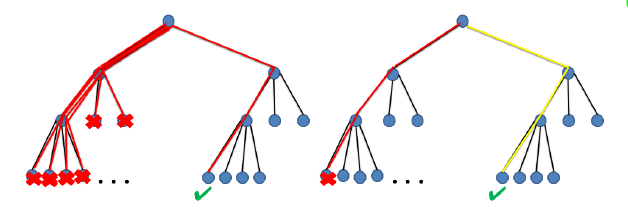
\includegraphics[width=1\textwidth]{images/search_parallel.png}
    \caption{Превенција узалудне претраге стабла уз помоћ паралелизације}
    \label{fig:search_parallel}
\end{figure}

\subsection{\textit{OpenMP} имплементација}\label{sec:mp_impl}

За разлику од постојећих решења која су се користила \textit{pthreads} \cite{pthreads} библиотеком, аутор је за имплементацију одабрао \textit{OpenMP} \cite{open_mp} ради декларативнијег приступа имплементацији.


\begin{listing}[H]
\inputminted{c}{kodovi/mp_search.c}
\caption{\textit{OpenMP} имплементација претраге}
\label{code:mp_search}
\end{listing}

За потребе паралелизације, петља унутар \textit{solve} функције која је служила за рекурзивну претрагу морала је подлећи одређеним модификацијама. Помоћу \textit{MP} директива, петља је паралелизована, тако да сада свака њена итерација која испробава један модел решења сада може да се извршава на засебној нити. Уместо да се резултат решења директно враћа из петље, сада се јавила потреба за дељеном променљивом \textit{finalResult} којој се приступа унутар критичне секције и уписује решење уколико се пронађе. Да би се одмах након проналаска решења прекинуо рад и свих осталих нити, уводи се још једна дељена променљива \textit{stopSignal}, чију вредност нит која је дошла до решења мења на \textit{true} и тако сигнализира свим осталим нитима да истог тренутка прекину са радом.

\subsection{\textit{OpenMP} имплементација употребом \textit{task}-ова}

Ова имплементација концептуално је слична \textit{MP} имплементацији преко примитива \ref{sec:mp_impl}. Разлика је у томе што сада само једна нит унутар петље креира \textit{task}-ове који се затим распоређују по свим нитима унутар паралелног региона \ref{code:mp_tasks_search}. Начин пропагације коначног решења и прекида рада свих осталих \textit{task}-ова остаје непромењен.

\begin{listing}[H]
\inputminted{c}{kodovi/mp_tasks_search.c}
\caption{\textit{OpenMP} имплементација претраге употребом \textit{task}-ова}
\label{code:mp_tasks_search}
\end{listing}

\subsection{\textit{OpenMPI} имплементација} 
Будући да се начин функционисања \textit{OpenMPI}-а \cite{open_mpi} разликује од \textit{OpenMP}-а, ова имплементација се знатно разликује од све три претходне.
Оно што разликује ову \textit{OpenMPI} имплементацију од постојећих је покушај делегирања посла једног процеса на све расположиве процесе, за разлику од тренутних имплементација где би процес био у могућности да половину свог посла делегира само суседном процесу (посматрајући \textit{id} процеса).\\

\subsubsection{Структуре података}

Поред постојећих структура података за ћелију и читаву судоку матрицу додат је низ \textit{unsigned} вредности \textit{availabilities} величине једнаке броју процеса који води рачуна о заузетости сваког од процеса. Такође било је потребно дефинисати нове \textit{MPI} типове података за размену ћелија и информација о доступности процеса између процеса \ref{code:mpi_structures}, као и написати помоћне функције за постављање судоку матрице у континуалан део меморије како би се она могла размењивати између процеса.

\begin{listing}[H]
\inputminted{c}{kodovi/mpi_structures.c}
\caption{Додатне структуре података}
\label{code:mpi_structures}
\end{listing}

\subsubsection{Хијерархија процеса и начин рада}

Читав рад заснива се на бесконачној петљи у којој се сви процеси налазе и чекају да им посао буде делегиран. Изузетак је петља са рангом 0, која је проглашена координатором који се бави вођењем евиденције о заузетости процеса и обавештавањем других процеса о тој информацији, као и очекивању коначног решења и финализацији алгоритма. Алгоритам почиње тако што координатор процес покушава пропагацију ограничења и ако из првог покушаја успе да реши загонетку одмах завршава програм, у супротном судоку матрицу са до тог тренутка максимално прорпагираним ограничењима прослеђује као задатак за решавање процесу 1 \ref{code:mpi_initial_cp}. 

\begin{listing}[H]
\inputminted{c}{kodovi/mpi_initial_cp.c}
\caption{Иницијална пропагација ограничења}
\label{code:mpi_initial_cp}
\end{listing}

Будући да би сви процеси требали да се баве својим задацима и асинхроно ослушкују да ли им је стигла нека порука, на разним местима у коду налази се слична конструкција која је приказана у коду \ref{code:mpi_message_waiting}. Сваки процес на почетку петље проверава да ли му је упућена нека порука и уколико јесте на основу њеног тага, одређује да ли се ради о поруци за завршетак процеса, поруци о прослеђеној матрици (решеној или спремној за обраду) или поруци за освежавање информације о доступности процеса.

\begin{listing}[H]
\inputminted{c}{kodovi/mpi_message_waiting.c}
\caption{Пример конструкције за  асинхроно ослушкивање порука}
\label{code:mpi_message_waiting}
\end{listing}

У код \textit{solve} методе коју позивају процеси када добију матрицу за обраду додато је неколико нових делова. На самом почетку ажурира се листа доступних процеса за делегирање посла и након пропагације ограничења пре него што се уђе у петљу за претрагу простора могућих ограничења процес прво делегира део посла свим доступним процесима\ref{code:mpi_job_delegation}. Након делегације посла, процес ће истражити преостале случајеве који нису делегирани. У случају проналаска решења оно се шаље директно координаторском процесу и завршава се програм.

\begin{listing}[H]
\inputminted{c}{kodovi/mpi_job_delegation.c}
\caption{Делегирање дела посла слободним процесима}
\label{code:mpi_job_delegation}
\end{listing}